Одной из наиболее проработанных научных психологический теорий интеллектуального развития 
является теория когнитивного развития, разработанная Жаном Пиаже \cite{piaget1952origins}.
Когнитивное развитие происходит в форме стадий, соответствующих развитию интеллектуальных
способностей. Таковыми являются все виды мыслительных процессов, таких как восприятие,
память, формирование понятий, решение задач, воображение и логика.

Этапы развития детской психики по Жану Пиаже:

\begin{enumerate}
    \item сенсомоторный интеллект;
    \item дооперациональные представления;
    \item период конкретных операций;
    \item конкретное и абстрактное логическое мышление. 
\end{enumerate}

Пиаже обосновывает свою теорию этичными экспериментами, легко доступными к воспроизведению педагогам.

\begin{figure}[h]
    \centering
    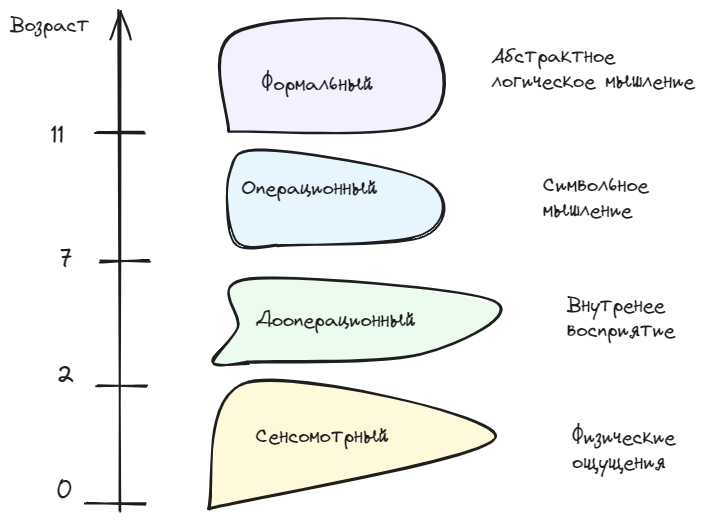
\includegraphics[width=0.5\textwidth]{assets/pedagogic/psy/piage.excalidraw.png}
    \caption{Этапы развития детской психики по Жану Пиаже \cite{piaget1952origins}.}
    \label{piage}
\end{figure}



Л. С. Выготский оспаривает этот подход, приводя в пример детей, которые в ходе занятий со взрослыми продемонстрировали
высокий уровень освоения шахмат \ref{proximal_growth}. Выполненные Выготским
эксперименты стали основой направления культурно-исторической психологии, признанной в мировой психологии.
Согласно Выготскому образование имеет социальный и целенаправленный характер, связанное с развитием
\textit{высших психических функции} --- сложных самоорганизующихся процессов в деятельности человека, 
опосредованных знаками по своему строению и произвольных по способу своего осуществления. В качестве таких навыков Выготский
определяет мышление, речь, произвольное внимание, волю, воображение и др.

\textit{Определение:} \textbf{Зона ближайшего развития} --- расхождение между уровнем актуального психического развития ребёнка
 и уровнем его потенциального развития, достигаемого при решении задач в сотрудничестве со взрослым или сверстниками. 

 \begin{figure}[h]
    \centering
    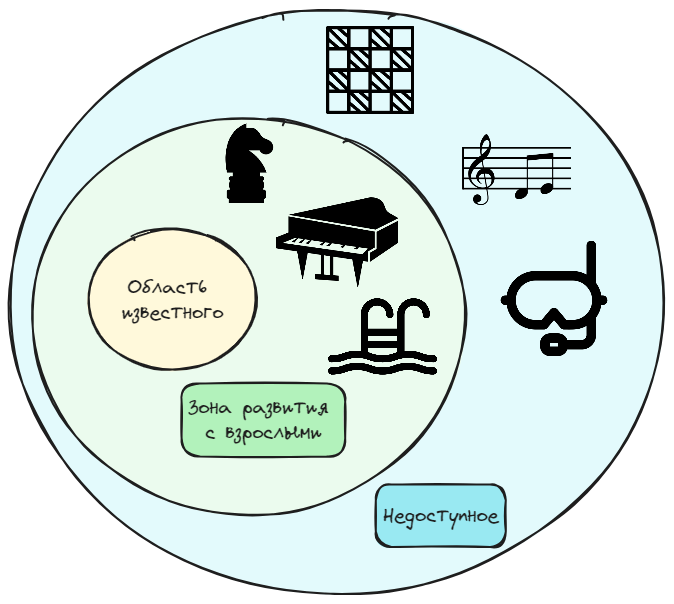
\includegraphics[width=0.5\textwidth]{assets/pedagogic/psy/proximal_growth.excalidraw.png}
    \caption{Иллюстрация зоны ближайшего развития.}
    \label{proximal_growth}
\end{figure}


Согласно Выготскому ключевым для образовании является процесс рефлексии учащегося.
Такой процесс включает в себя осознанный анализ своего учебного опыта, рассмотрение своих мыслей, чувств и действий в контексте обучения. 
Механизмом рефлексии является \textit{интериоризация}. Процесс заключается в переходе внешней речи во внутренний способ мышления.
Отметим, что процесс возможен когда ребёнок уже способен планировать свою деятельность. 
 
\begin{figure}[h]
    \centering
    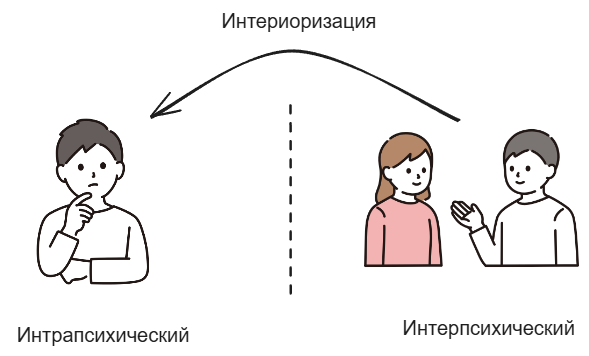
\includegraphics[width=0.5\textwidth]{assets/pedagogic/psy/reflection.excalidraw.png}
    \caption{Рефлексия по Выготскому \cite{выготский2014мышление}.}
    \label{reflection}
\end{figure}
 
 Рефлексия способствует развитию метакогнитивных навыков:
  \begin{itemize}
     \item оценки своей деятельности и планирования;
     \item осознания ценности знания и социума;
     \item ведения высшей когнитивной деятельности по организации социальной деятельности.
 \end{itemize}
Такие навыки позволяют справляться с практическими заданиями, обучать и осваивать неизвестные области знания,
выявлять пробелы в знаниях и развивать критическое мышление.

\textit{Определение:} \textbf{Поток} --- это состояние сознания, характеризующееся полной вовлеченностью и концентрацией
на текущей деятельности, сопровождающееся ощущением контроля, потерей чувства времени и высокой внутренней мотивацией.

Теория потока активно используется в играх \cite{chen2007flow} и программах непрерывного обучения \cite{jarvis2009routledge} для
задания оптимальной сложности образовательной программы.

\begin{figure}[h]
    \centering
    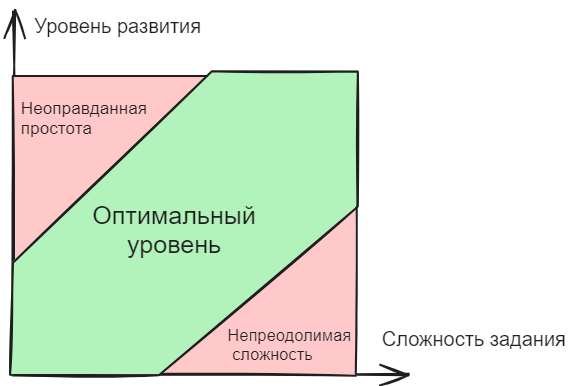
\includegraphics[width=0.5\textwidth]{assets/pedagogic/psy/flow.excalidraw.png}
    \caption{Рефлексия по Выготскому \cite{выготский2014мышление}.}
    \label{reflection}
\end{figure}

Характеристиками потока согласно \cite{csikszentmihalyi2005flow} являются:
 \begin{itemize}
    \item Ясные цели и обратная связь: Деятельность имеет чёткие цели и предоставляет немедленную обратную связь.
    \item Баланс между сложностью задачи и навыками: Задача должна быть достаточно сложной, чтобы представлять собой вызов, но при этом соответствовать уровню навыков человека, чтобы избегать скуки и тревоги.
    \item Слияние действия и сознания: Человек настолько поглощён деятельностью, что все его действия становятся почти автоматическими и интуитивными.
    \item Потеря самосознания: В потоке человек забывает о себе, своих заботах и тревогах, полностью сосредоточившись на задаче.
    \item Искажение восприятия времени: Время может казаться летящим быстро или, наоборот, замедляться; часы могут пройти как минуты
\end{itemize}


\textit{Определение:} \textbf{Гипотеза о врожденных знаниях}(\textit{англ.} Innateness hypothesis) --- теория в лингвистике и когнитивной науке,
 которая утверждает, что способность к языку является врождённой характеристикой человеческого мозга. 

Гипотеза постулирует наличие:
\begin{itemize}
    \item врождённого языкового аппарата, способствующего естественному освоению языка;
    \item универсальной грамматики, состоящей из набора грамматических принципов и структур, присутствующих во всех языках и врождённых для каждого человека;
    \item основных аспектов языковой способности, являющихся врождёнными и не зависящими от окружающей среды.
\end{itemize}

Гипотеза имеет статистические подтверждения описанные в работах Р. Номски, использовавшего статистический аппарат синтаксических деревьев для анализа массивного
корпуса естественного языка \cite{everaert2015structures}\cite{montague1970universal}.




